%%%%%%%%%%%%%%%%%%%%%%%%%%%%%%%%%%%%%%%%%%%%%%%%%%%%%%%%%%%%%%%%%%%%%%%%%
\documentclass[12pt]{article}
%\usepackage[spanish]{babel}
\textwidth     =  7.0in
\textheight    =  9.0in
\oddsidemargin = -0.2in
\topmargin     = -.5in

%%%%%%%%%%%%%%%%%%%%%%%%%%%%%%%%%%%%%%%%%%%%%%%%%%%%%%%%%%%%%%%%%%%%%%%%

\usepackage{amsmath, amsthm, amssymb, latexsym}
\usepackage[spanish]{babel}
\usepackage[utf8]{inputenc}
\usepackage{hyperref}
\usepackage{graphicx}

\newtheorem{lma}{Lema}
\newtheorem{thm}{Teorema}
\newtheorem{prb}{Prueba}
%----------------------------------------------------------------------
%
% Archivo LaTeX para el proyecto de reconocimiento de patrones
%
% curso:       Modelos matematicos y numericos
% instructor:  Jose Luis Morales
%              Departamento de Matematicas
%              I T A M
%              agosto 2015
%
%----------------------------------------------------------------------

\newcommand{\real}{\mathbb{R}}
\newcommand{\complex}{\mathbb{C}}
\newcommand{\feal}{\mathbb{F}}
\newcommand{\ul}{\underline}
%
\newcommand{\noi}{\noindent}
\newcommand{\pa}{\partial}
%
\newcommand{\bea}{\begin{eqnarray}}
\newcommand{\eea}{\end{eqnarray}}
%
\newcommand{\beas}{\begin{eqnarray*}}
\newcommand{\eeas}{\end{eqnarray*}}
%
\newcommand{\non}{\nonumber}
%
\newcommand{\bit}{\begin{itemize}}
\newcommand{\eit}{\end{itemize}}
%
\newcommand{\bee}{\begin{enumerate}}
\newcommand{\eee}{\end{enumerate}}
%
\newcommand{\bed}{\begin{description}}
\newcommand{\edd}{\end{description}}
%
\newcommand{\bec}{\begin{center}}
\newcommand{\edc}{\end{center}}
%
\begin{document}
\title{\textbf{Reconocimiento de dígitos mediante \\Descomposición en Valores Singulares (DVS)}}
\author{Modelos matemáticos y numéricos}
\date{Jos\'e Manuel Proudinat Silva}
\maketitle

%%%%%%%%%%%%%%%%%%%%%%%%%%%%%%%%%%%%%%%%%%%%%%%%%%%%%%%%%%%%%%%%%%%%%%%%

\section{Introducción}

El objetivo de este documento es presentar los fundamentos y resultados obtenidos al crear un clasificador que pudiera reconocer un dígito mediante la lectura de una imagen del mismo escrito a mano. 

Para ello se utilizó una muestra de la base de datos MNIST, la cual contiene un conjunto de 5000 observaciones, 500 observaciones por cada dígito, además del valor real del mismo. Cada una de ellas consiste de un vector elemento de $\real^{400}$, el cual representa la intensidad de cada uno de los pixeles de la imagen del dígito en escala de grises.

Este problema es de gran relevancia en varios sentidos. Desde una perspectiva académica, nos permite ver una aplicación real que envuelve un variado conjunto de ramas de las matemáticas, entre ellas el álgebra lineal y el análisis numérico. Desde un plano práctico, el reconocimiento de imágenes involucra muchas disciplinas en la industria y el gobierno, como lo es la seguridad, conversión de documentos, entre otros.

Para clasificar los dígitos, se proyectaron sus vectores de datos sobre el espacio generado por los primeros $k$ (este parámetro fue variado durante la experimentación) valores singulares del conjunto de datos de entrenamiento para cada dígito. La predicción se daba según el espacio en que se obtuviera el menor residuo entre el vector original y el proyectado. Más adelante se explicará a mayor detalle este proceso.

%%%%%%%%%%%%%%%%%%%%%%%%%%%%%%%%%%%%%%%%%%%%%%%%%%%%%%%%%%%%%%%%%%%%%%%%


%%%%%%%%%%%%%%%%%%%%%%%%%%%%%%%%%%%%%%%%%%%%%%%%%%%%%%%%%%%%%%%%%%%%%%%%

\section{Descomposición en Valores Singulares}

\subsection{Existencia de la DVS}

\begin{thm} [Descomposici\'on en valores singulares] \label{svd} 
 
 Si $A$ es una matriz real de $m \times n$, entonces existen matrices ortogonales
\[
   U \in \real^{m \times m}, \quad
   V = \in \real^{n \times n} 
\]
tales que 
\[
  U^TAV = \Sigma = {\rm diag}(\sigma_1, \ldots, \sigma_p) \in \real^{m \times n}, \quad   p = \min \{m,n\}
\]
en donde $\sigma_1 \ge \sigma_2 \ge \ldots \ge \sigma_p \ge 0$.
\end{thm}

\begin{prb}

\bigskip

Sea $S = \{ x \in \real^n : ||x||_2 = 1 \}$. Definimos $\sigma_1 = ||A||_2 = sup_{x \in S}||Ax||_2$ y tomamos la función $f:S\rightarrow \real$ dada por $f(x) = ||Ax||_2$. Como $f$ es una función continua (pues las transformaciones lineales y la norma 2 son continuas) y $S$ es un conjunto compacto (es una bola cerrada de radio 1). Entonces por el teorema del valor extremo, existe un máximo de $f$ en $S$, es decir, existe $v_1 \in S$ tal que $||Av_1||_2 = \sigma_1$. Denotamos $u_1 = \frac{1}{\sigma_1}Av_1$.

Construimos una base ortonormal $\{v_j\}$ para $\real^n$ a partir de $v_1$ y una base ortonormal $\{u_j\}$ para $\real^m$ a partir de $u_1$. Tomamos $U_1 = [u_1 \dots u_m]$ y $V_1 = [v_1 \dots v_m]$ entonces:

$$
U_1^TAV_1 = \left [ 
    \begin{array}{cc}  
    \sigma_1 & w^T \\
    0 & B  
    \end{array} 
    \right ] = A_1
$$

en donde $w \in \real^{n-1}$ y $B \in \real^{(m-1) \times (n-1)}$;
de la desigualdad 
\[
   \left |\left | A_1   \left [ \begin{array}{c} \sigma_1 \\ w \end{array} \right ] \right |\right|_2^2  \ge ( \sigma_1^2 + w^Tw )^2
\]
podemos concluir que $||A_1||_2^2 \ge  \sigma^2 + w^Tw$. Sin embargo $\sigma_1^2 = ||A||_2^2 = ||A_1||_2^2$ (ya que $U$ y $V$ son ortonormales), por lo tanto $w=0$. Es decir que $A_1$ tiene la estructura diagonal por bloques
\[
 A_1 = \left [ \begin{array}{cc}  \sigma_1 &    0 \\
                                         0   & B  
                   \end{array} 
       \right ].
\]

Repetimos el proceso para la matriz $B$ y las consecuentas submatrices no diagonales consecuentes hasta completar el proceso obteniendo $U_2, \dots, U_p$ y $V_2, \dots, V_p$ para construir $U$ y $V$ tal que:

$$U^TAV = \Sigma = {\rm diag}(\sigma_1, \ldots, \sigma_p).$$

\hfill $\square$

\end{prb}

\subsection{Propiedades}

La DVS revela pr\'acticamente toda la estructura algebraica de una matriz. Por ejemplo:
\begin{enumerate}
  \item Los valores singulares de $A$ son las longitudes de los semi ejes del hiperelipsoide 
        \[
           H = \left \{ Ax : ||x||_2 =1 \right \}
        \]
         definido por $A$.
  \item Si definimos $r$ como 
  \[
     \sigma_1 \ge \cdots \sigma_r > \sigma_{r+1} = \cdots = \sigma_p = 0,
  \]
  entonces 
    \begin{enumerate}
     \item $\mbox{rango}(A) = r$
     \item $K(A) = \mbox{gen} \left \{ v_{r+1}, \ldots, v_n \right \}$
     \item $R(A) = \mbox{gen} \left \{ u_1, \ldots, u_r \right \}$
    \end{enumerate}
  \item La matriz $A$ se puede representar como una suma de matrices de rango 1 (desarrollo DVS)
         \begin{eqnarray} \label{suma}
            A = \sum_{i=1}^r \sigma_i u_i v_i^T.
         \end{eqnarray}
  \item Diversas relaciones entre  $||A||_{\rm F}$ y $||A||_2$
        \begin{enumerate}
         \item $||A||_{\rm F} = \sigma_1^2 + \cdots + \sigma_p^2$, \quad $p = \min\{m,n\}$
         \item $||A||_2 = \sigma_1$
         \item $\displaystyle{ \min_{||x||_2 = 1} ||Ax||_2 = \sigma_n}$, \quad $(m \ge n)$.
        \end{enumerate}
\end{enumerate}


\subsection{Implementación numérica}

El algoritmo más utilizado para realizar esta descomposición de matrices (el cual está implementado en Matlab y Lapack) es una versión revisada del algoritmo presentado por Gloub y Van Loan. Esta versión revisada fue presentada por J. Demmel y W. Kahan en su artículo "Accurate Singular Values of Bidiagonal Matrices" (1990). La idea detrás del mismo la podemos ver en dos pasos: Primero, la matriz se reduce a una forma bidiagonal $B$ a través de transformaciones de Householder. Durante estas iteraciones podemos construir U y V multiplicando las matrices de rotación que surgen mientras iteramos. De esta forma llegamos a una descomposición de la forma $A=UBV^T$.

Finalmente comenzamos un proceso iterativo con la matriz bidiagonal en el cual vamos haciendo ceros los valores de $B$ que cumplan que $|b_{i,i+1}|\leq \epsilon(|b_{i,i}|+|b_{i+1,i+1}|).$ Partimos B en 3 bloques, tal que el tercer bloque sea diagonal y el segundo no tenga ceros en la diagonal superior. Si encontramos un cero en la diagonal del segundo bloque se aplican rotaciones de Givens, de tal forma que el segundo bloque siga siendo bidiagonal superior (Golub-Reinsch). Si no hay ceros, aplicamos otro subalgoritmo con rotaciones de Givens que van haciendo más pequeños los valores fuera de la diagonal de $B$ (Golub-Kahan). Iteramos hasta que B sea una matriz completamente diagonal.

Golub y Van Loan muestran en su libro "Matrix computation" que este algoritmo es de orden $\mathcal{O}(m^2n + n^3)$ si queremos hallar la descomposición completa.

%%%%%%%%%%%%%%%%%%%%%%%%%%%%%%%%%%%%%%%%%%%%%%%%%%%%%%%%%%%%%%%%%%%%%%%%

%%%%%%%%%%%%%%%%%%%%%%%%%%%%%%%%%%%%%%%%%%%%%%%%%%%%%%%%%%%%%%%%%%%%%%%%

\section{Problema de mínimos cuadrados}

Ahora mostraremos con argumentos de álgebra lineal como el problema de mínimos cuadrados $Ax=b$ tiene solución en $\bar x = (A^TA)^{-1}A^Tb$. Donde $A$ es una matriz de $m * n$ con $m \geq n$ de rango completo.

Como $A$ es de rango completo, entonces $A^TA$ es simétrica positiva definida, y por lo tanto es invertible.

Buscamos $\bar x$ tal que minimice el error dado por $r = b - A\bar x$. El cual en Álgebra Lineal se demuestra que está dada por la proyección en $A$ de $b$. Por lo cual tomando $A\bar x$ como la proyección, tenemos que esta debe ser ortogonal al residuo. Es decir, $(b - A\bar x)^TA\bar x = 0$. Con lo que llegamos a lo siguiente:

\begin{align*}
& (A\bar x)^T(b - A\bar x) = 0\\
\Leftrightarrow & \ \bar x^TA^Tb - \bar x^TA^TAx = 0\\
\Leftrightarrow & \ \bar x^T (A^Tb - A^TA\bar x) = 0\\
\Leftrightarrow & \ A^Tb - A^TA\bar x = 0\\
\Leftrightarrow & \ A^TA\bar x = A^Tb\\
\Leftrightarrow & \ \bar x = (A^TA)^{-1}A^Tb
\end{align*}

%%%%%%%%%%%%%%%%%%%%%%%%%%%%%%%%%%%%%%%%%%%%%%%%%%%%%%%%%%%%%%%%%%%%%%%%

%%%%%%%%%%%%%%%%%%%%%%%%%%%%%%%%%%%%%%%%%%%%%%%%%%%%%%%%%%%%%%%%%%%%%%%%

\section{Componentes principales y DVS}

A continuación haremos una interpretación del Análisis de Componentes Principales (ACP) tomando la idea de la Descomposición en Valores Singulares.

El ACP es un método de estadística multivariada en el cual se busca crear una combinación lineal de los vectores de datos de tal manera que esta represente el mayor porcentaje de la varianza de los datos. Recordemos que el ACP requiere que se calculen los valores propios y vectores propios de su matriz de covarianzas $XX^T$, donde $X$ es la matriz de datos. Pues se demuestra que éstos son los valores de máxima varianza obtenida, y sus valores propios representan las combinaciones lineales que permiten la reducción de dimensiones. Como la matriz de covarianzas es simétrica podemos hacer la descomposición espectral de la matriz:

$$XX^T = QDQ^T$$

Donde D es la matriz diagonal de valores propios y Q es una matriz ortogonal conteniedo a los vectores propios.

Usando la DVS de X podemos llegar a que:

\begin{align*}
XX^T = & \ (U\Sigma V^T)(U \Sigma V^T)^T\\
= & \ U \Sigma V^T V \Sigma U^T\\
= & \ U \Sigma^2 U^T
\end{align*}

De esta manera la interpretación es sencilla. Observamos que los cuadrados de los valores singulares de $X$ contenidos en $\Sigma$ representan la varianza que logra representar la combinación lineal de los datos dada por los vectores en $U$. Así observamos también que los vectores de $U$ representan las combinaciones lineales que nos dan las distintas reducciones de dimensiones que buscan representar lo máximo posible de la varianza total de los datos.


%%%%%%%%%%%%%%%%%%%%%%%%%%%%%%%%%%%%%%%%%%%%%%%%%%%%%%%%%%%%%%%%%%%%%%%%
\section{Aplicación al reconocimiento de dígitos}

Consideremos un d\'{\i}gito particular, digamos $d \in \{0,1, \ldots, 9\}$. Si obtenemos la DVS de $A^d$, entonces tenemos: 
         \[
            A^d = \sum_{i=1}^r \sigma_i u_i v_i^T.
         \]
lo que indica que cada columna de $A^d$, denotada como $a_j$,  se puede expresar como
\[
      a_j = \sum_{i=1}^m (\sigma_i v_{ij}) u_i,
\]
en donde $v_{ij}$ es la $j$-\'esima componente del vector $v_i$. La expresi\'on anterior sugiere que cada columna se puede aproximar por los primeros $K$ t\'erminos de la suma, es decir
\[
       a_j \approx \sum_{i=1}^K (\sigma_i v_{ij}) u_i.
\]
Notar que los primeros vectores singulares de $A^d$ contienen la {\em informaci\'on dominante}. Pues podemos ver que la DVS es, en este sentido, similar a la reducción de dimensiones implementada en los algoritmos de Análisis de Componentes Principales (como se menciona en el documento complementario de ejercicios). Es por eso que los primeros valores singulares contienen un alto porcentaje de la varianza de los datos, es decir la información que éstos contienen.

Ahora podemos identificar un d\'{\i}gito desconocido, digamos $z$, resolviendo el siguiente problema de m\'{\i}nimos cuadrados (MC).
\[
    \mbox{minimizar}  \quad || z - U_K \alpha ||_2^2,
\]
en donde $U_K$ es la submatriz de $U$ formada por los primeros $K$ vectores singulares. La soluci\'on del problema de MC es 
\[
    \alpha = U_K^Tz,
\]
mientras que la norma del residuo es 
\begin{eqnarray}  \label{MC}
  ||r(z)||_2 = || z - U_KU_K^Tz||_2
\end{eqnarray}
 Es inmediato concluir que si $||r(z)||_2$ es muy peque\~na, entonces probablemente $z = d$.
 
Para la implementación del algoritmo se desarrolló código en Matlab atacando el problema desde la perspectiva de la programación funcional y programación orientada a objetos. Finalmente se decidió utilizar el enfoque orientado a objetos pues minimizaba el uso de memoria de la máquina y tiempo en ejecución.

El código completo es abierto y se puede encontrar en el siguiente repositorio:\\ \url{https://github.com/JosmanPS/Modelos-Matematicos-y-Numericos/tree/master/Proyecto_1}.

%%%%%%%%%%%%%%%%%%%%%%%%%%%%%%%%%%%%%%%%%%%%%%%%%%%%%%%%%%%%%%%%%%%%%%%%

%%%%%%%%%%%%%%%%%%%%%%%%%%%%%%%%%%%%%%%%%%%%%%%%%%%%%%%%%%%%%%%%%%%%%%%%

\section{Resultados}

Se hicieron 100 clasificaciones para diferentes números de valores singulares (desde uno hasta veinte). Con esto se hizo una estimación de su tasa de acierto de entrenamiento y de prueba. Ésta última distinción se hizo para poder visualizar el poder de predicción de este método ante valores fuera de su conjunto de datos de entrenamiento. En los siguientes cuadros se pueden visualizar los resultados obtenidos.

\begin{table}[H]
\centering
\begin{tabular}{rrr}
  \hline
 k & entrenamiento & prueba \\ 
  \hline
1 & 0.78 & 0.86 \\ 
  2 & 0.86 & 0.92 \\ 
  3 & 0.87 & 0.95 \\ 
  4 & 0.90 & 0.87 \\ 
  5 & 0.95 & 0.89 \\ 
  6 & 0.93 & 0.90 \\ 
  7 & 0.91 & 0.96 \\ 
  8 & 0.99 & 0.97 \\ 
  9 & 0.93 & 0.92 \\ 
  10 & 0.96 & 0.91 \\ 
  11 & 0.96 & 0.93 \\ 
  12 & 0.96 & 0.92 \\ 
  13 & 0.93 & 0.96 \\ 
  14 & 0.98 & 0.92 \\ 
  15 & 0.99 & 0.94 \\ 
  16 & 0.97 & 0.95 \\ 
  17 & 0.95 & 0.93 \\ 
  18 & 0.91 & 0.93 \\ 
  19 & 0.97 & 0.92 \\ 
  20 & 0.95 & 0.97 \\ 
   \hline
\end{tabular}
\caption{\label{fig:p1}Tasa de acierto para k valores singulares.}
\end{table}

\begin{figure}[H]
\centering
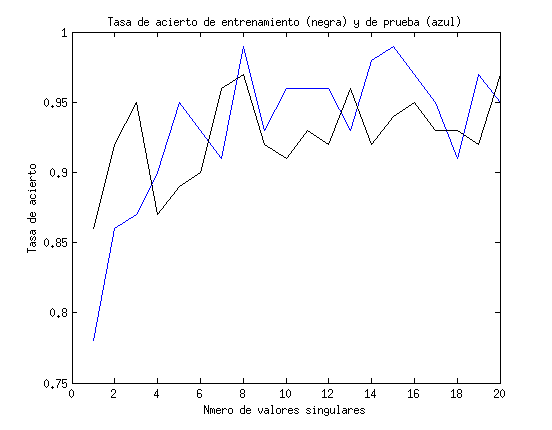
\includegraphics[width=0.5\textwidth]{tasa_acierto.png}
\caption{\label{fig:p2}Ecuación problema 3.}
\end{figure}

Podemos observar que sí hay un mejor rendimiento mientras aumentamos el número de valores singulares utilizados en la proyección, sin embargo no es tan significativo, pues desde el primer valor ya estamos tomando la mayor parte de la información contenida en las imágenes. Además vemos que no hay gran diferencia entre los aciertos de entrenamiento y los de prueba por lo que podemos asumir que este método tiene un buen poder de predicción incluso para datos fuera de su muestra de entrenamiento.

\thebibliography{99}

\item Gene H. Golub & Charles F. Van Loan, \textit{Matrix computations}. 3th edition. Josh Hopkins University. 1996.

\item Alan Kaylor Cline & Inderjit S. Dhillon, \textit{Computation of the Singular Value Decomposition}. \textit{Handbook of Linear Algebra}. Discrete mathematics and its application. Series editor KENNETH H. ROSEN. Chapman & Hall/CRC.2007.


%%%%%%%%%%%%%%%%%%%%%%%%%%%%%%%%%%%%%%%%%%%%%%%%%%%%%%%%%%%%%%%%%%%%%%%%


\end{document}
